\section{Experiments}\label{sec:experiments}

% \begin{itemize}
%     \item \mdeff{In general, we should try to make the text in figures larger. A trick I use in matplotlib is to lower the figure size, e.g., \texttt{fig = %plt.figure(figsize=(4, 4))}}.done
% \end{itemize}

% Feasibility (one component).
We started by evaluating whether orientation recovery \eqnref{orientation-recovery} was feasible assuming perfect distances, and how it was affected by errors in distance estimations (\secref{results:orientation-recovery:sensitivity}).
We then learned to estimate distances \eqnref{distance-learning} and evaluated how accurate they were (\secref{results:distance-estimation:learned}).
% Real stuff (the two steps together).
Following this, we evaluated the robustness of distance learning to perturbations of the projections and its transferability to unseen proteins (\secref{results:distance-estimation:sensitivity}).
Finally, we ran the whole machinery to assess how well orientations could be recovered from distances estimated by the trained SiameseNN (\secref{results:orientation-recovery:reconstruction}).

%%%%%%%%%%%%%%%%%%%%%%%%%%%%%%%%%%%%%%%%%%%%%%%%%%%%%%%%%%%%%%%%%%%%%%%%%%%%%%%%%%%%%%%

\subsection{Experimental conditions}\label{sec:results:data}

\paragraph{Density maps.}
We considered two proteins (\figref{pdb-proteins}): the $\beta$-galactosidase, a protein with a dihedral (D2) symmetry, and the lambda excision HJ intermediate (HJI), an asymmetric protein with local cyclic (C1) symmetry.
Their deposited PDB atomic models are \texttt{5a1a}~\cite{bartesaghi2015betagal} and \texttt{5j0n}~\cite{laxmikanthan2016structure}, respectively.
For each atomic model, we generated the density map by fitting a 5\AA\ map in Chimera~\cite{pettersen2004ucsf}; this gave us a volume of $110 \times 155 \times 199$ voxels for the $\beta$-galactosidase, and $69 \times 57 \times 75$ voxels for the HJI\@.
% -sized volume

\begin{figure}[ht!]
    \centering
    \begin{minipage}[b]{0.45\linewidth}
        \centering
        \begin{subfigure}[b]{0.46\linewidth}
            \centering
            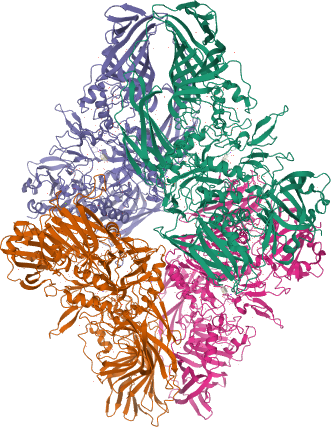
\includegraphics[height=3cm]{figures/5a1a_pdb.png}
            \caption{Atomic model of \texttt{5a1a}.}
        \end{subfigure}
        \hfill
        \begin{subfigure}[b]{0.46\linewidth}
            \centering
            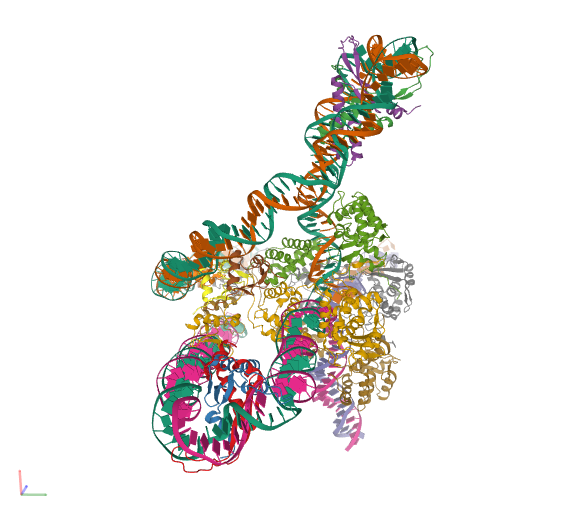
\includegraphics[height=3cm]{figures/5j0n_pdb.png}
            \caption{Atomic model of \texttt{5j0n}.}
        \end{subfigure}
        \\ \vspace{0.5em}
        \begin{subfigure}[b]{0.46\linewidth}
            \centering
            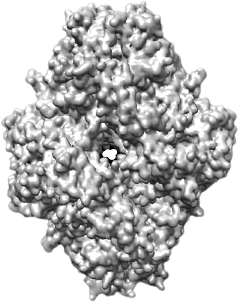
\includegraphics[height=3cm]{figures/5a1a_5A_.png}
            \caption{Density map $\x$ of \texttt{5a1a}.}
        \end{subfigure}
        \hfill
        \begin{subfigure}[b]{0.46\linewidth}
            \centering
            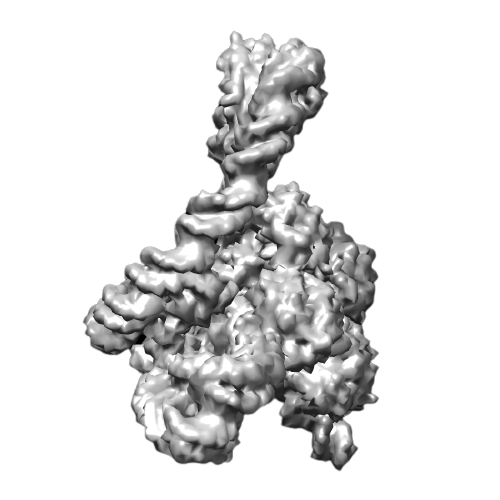
\includegraphics[height=3cm]{figures/5j0n_5A_.png}
            \caption{Density map $\x$ of \texttt{5j0n}.}
        \end{subfigure}
        \caption{%
            Two proteins with different symmetries.
            %The $\beta$-galactosidase (\texttt{5a1a}) and the lambda excision HJ intermediate (\texttt{5j0n}).
        }\label{fig:pdb-proteins}
    \end{minipage}
    \hfill
    \begin{minipage}[b]{0.45\linewidth}
        \centering
        \begin{subfigure}[b]{0.49\linewidth}
            \centering
            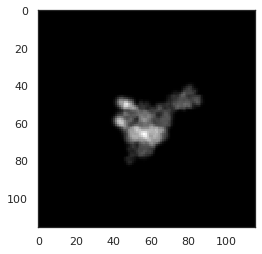
\includegraphics[height=3cm]{figures/5j0n_noise0}
            \caption{$\mathbf{P}_{\bth} \mathbf{x}$}
        \end{subfigure}
        \hfill
        \begin{subfigure}[b]{0.49\linewidth}
            \centering
            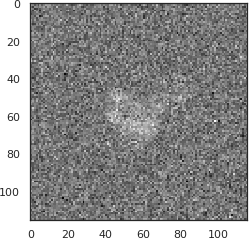
\includegraphics[height=3cm]{figures/5j0n_noise16}
            \caption{$\mathbf{P}_{\bth} \mathbf{x} + \mathbf{n}$}
    %, \; \mathbf{n} \sim \mathcal{N}(0, 16\mathbf{I})$}
        \end{subfigure}
        \\ \vspace{0.5em}
        \begin{subfigure}[b]{0.49\linewidth}
            \centering
            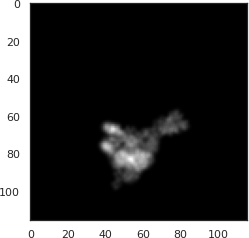
\includegraphics[height=3cm]{figures/5j0n_translated}
            \caption{$\mathbf{S}_{\mathbf{t}} \mathbf{P}_{\bth} \mathbf{x}$}
        \end{subfigure}
        \hfill
        \begin{subfigure}[b]{0.49\linewidth}
            \centering
            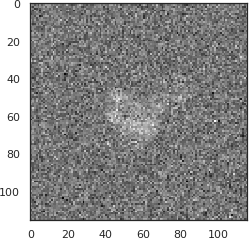
\includegraphics[height=3cm]{figures/5j0n_noise16_translated}
            \caption{$\mathbf{S}_{\mathbf{t}} \mathbf{P}_{\bth} \mathbf{x} + \mathbf{n}$}
        \end{subfigure}
        \caption{%
            Example projections of \texttt{5j0n}.
            % (a)~unperturbed, (b)~noisy, (c)~shifted, (d)~noisy and shifted.
        }\label{fig:different-projections}
    \end{minipage}
\end{figure}

\paragraph{Simulated projections.}
Using the ASTRA projector~\cite{van2015astra}, we generated $P=5,000$ synthetic projections of $275 \times 275$ pixels for \texttt{5a1a} and $116 \times 116$ pixels for \texttt{5j0n}.
\mdeff{That's not a uniform sampling of $\SO(3)$. Shall we mention it? Argue for it? The distribution over orientations induces the distribution over distances.}
Orientations were obtained by uniformly sampling the Euler angles $\bth = (\theta_1,\theta_2,\theta_3)$.
\mdeff{Consistency: we used $\bth=(\theta_3,\theta_2,\theta_1)$ in \secref{method:orientation-representation} and \figref{imaging-geometry}. $(\theta_3,\theta_2,\theta_1)$ indicates that $\theta_1$ is the first rotation (and $\theta_3$ is the in-plane) via $\mathbf{R}_{\theta_3}\mathbf{R}_{\theta_2}\mathbf{R}_{\theta_1}$. But if there's a standard in the field we should use it. Either way, please update the notation everywhere.}
As projections are made by integrating through the 3D volume, projections from opposed directions $(\theta_2,\theta_1)$ are mirrors of each other---preventing cryo-EM reconstructions to resolve chirality\footnote{A protein is chiral if it cannot be superposed on its mirror image by any combination of translations or rotations.}~\todo{[ref or common knowledge?]}.
%\mdeff{Not only a rotation, but an integration through $z_3$. (As opposed projections are mirrored, we cannot resolve chirality. Projecting looses global orientation, integrating looses chirality.)}
% "fundamental issue with reconstruction in cryoEM in general."
% at high resolutions, the handedness can be determined by the chirality of alpha helices
% https://discuss.cryosparc.com/t/ab-initio-reconstruction-chirality-issue/2202
%Hence, we only sampled orientations from half the directions.
% it was sufficient to only sample half the $\mathbb{S}^2$ sphere parametrized by $(\theta_1,\theta_2)$.
It was hence sufficient to only sample half the directions \todo{$\theta_1 \in [0, \pi[ \; \subset [0, 2\pi[$} (\figref{imaging-geometry}). % for \texttt{5j0n}
% half coverage of the direction sphere
\mdeff{Did we try distance learning and estimation on full coverage of \texttt{5j0n}? I remember we first believed opposed projections would be identical. But as they are mirrored, the SiameseNN should be able to distinguish them.}
That is the kind of physical knowledge that should ideally be built into the SiameseNN architecture, as we did to get invariance to off-centering shifts (\secref{method:distance-learning}).

Symmetries are problematic to learn distances: two projections can be identical while not having been acquired from the same orientation---breaking an axiom of proper distance functions.
\figref{euclidean-not-robust:5a1a} illustrates the phenomenon.
For this reason, we further restricted orientations to \todo{$(\theta_3,\theta_2,\theta_1) \in \dots$} for \texttt{5a1a}.
Note that symmetries aren't an issue when estimating distances, recovering orientations, and reconstructing.
Projections acquired from symmetric parts of the protein would group together, indicating the symmetries.
The reconstructed parts can then be copied over.
\todo{Write better.}
% i.e., it is composed of four identical sub-units with two rotations of magnitude $\pi$ radians around the first axis followed by $\pi$ radians rotation around second axis, as illustrated and explained in~\cite{symmetry_in_protein,symmetry,scipion-em-github, rcsb-symmetry-view, EmpereurMot2019GeometricDO}.

We then perturbed the measurements with different levels of additive Gaussian noise~\cite{sorzano2004normalizing,shigematsu2013noise} and off-centering shifts. %, (iii) inclusion of the effects of the point-spread functions (PSF).
%The mathematical formulation of these three components is given in \eqnref{imaging-model}.
\figref{different-projections} displays samples of the simulated (perturbed) projections.

% From projections to pairs and subsets (which are used for distance learning and orientation recovery).
\paragraph{Splitting of datasets.}
For each protein, we split the projections into training, validation, and test subsets; and created \textit{disjoint} pairs of projections from each (\tabref{dataset}).
% which are used as input to the SiameseNN, and as output their respective quaternion distances (calculated from their orientations);
The training and validation sets were used to train and evaluate the SiameseNN, while the test set was used to evaluate orientation recovery given a trained SiameseNN.
%to ensure that it did not include any projection that was previously seen during the distance learning.
Note that we split the $P=5,000$ projections, not the $P^2 = 25 \times 10^6$ possible pairs, to ensure we evaluate generalization to unseen projections.
%some of the projections appearing in pairs in the training dataset can appear in pairs in the other datasets.
We further sampled $1\%$ of the training and validation pairs such that the distribution over distances was uniform (independently from the distribution over orientations) \mdeff{True for all experiments?}.
%\mdeff{It seems arbitrary to artificially limit the pairs to $1\%$, and we'd see more combinations instead of seeing $150$ times the same pairs.}
The goal was to uniformly spread the distance estimation error over the range of distances.
The error would otherwise concentrate on the extremities as distances are concentrated in the middle.
%\mdeff{So those pairs are sampled from $63,126$ pairs from the training dataset, rather than the $P^2$ possible pairs? If true, we should motivate somewhere why we limit our training dataset.}
%We restricted the size of our training and validation datasets due to Google Colaboratory\footnote{A hosted Jupyter notebook service from Google Research with resources that are not guaranteed and not unlimited.} training time limit of 12 hours.
% \mdeff{No. 100 epochs over 1% takes the same time as 1 epoch over 100%.}

\paragraph{Optimization settings.}
\todo{Jelena: check the settings, make sure they are used for all experiments, and add anything missing?}
We optimized \eqnref{distance-learning} with the RMSProp optimizer~\cite{tieleman2012rmsprop} and a learning rate of $10^{-3}$ for $150$ epochs.
With batches of $256$ pairs, that was $247$ steps per epoch for the training sets and $28$ for the validation sets (\tabref{dataset}).
Training took about 6 hours \mdeff{correct?} on a single GPU\@.
% 2.6 to 9.3 hours depending on available resources.
% \mdeff{We just want a ball-park (e.g., not a day or a week).}
We optimized \eqnref{orientation-recovery} with the Adam optimizer~\cite{kingma2014adam} and a learning rate of $0.5$ until convergence on batches of $256$ pairs sampled from the test sets (\tabref{dataset}).
\todo{Jelena: runtime estimation?}
We optimized \eqnref{orientation-recovery-error} with the FTRL optimizer~\cite{mcmahan2013ftrl}, a learning rate of $2$, and a learning rate power of $-2$ on batches of $256$ orientations sampled from the test sets (\tabref{dataset}).
We reported the lowest of 6 runs (3 per value of $m$) of 300 steps each.
\todo{Jelena: runtime estimation?}
% ($\sim$ 50 minutes in the best resource availability setting)

%%%%%%%%%%%%%%%%%%%%%%%%%%%%%%%%%%%%%%%%%%%%%%%%%%%%%%%%%%%%%%%%%%%%%%%%%%%%%%%%%%%%%%%

%\subsubsection{Robustness of Recovery to Additive Errors on the Relative Distances}
\subsection{Sensitivity of orientation recovery to errors in distance estimation}\label{sec:results:orientation-recovery:sensitivity}

%\mdeff{Story: (i) orientation recovery error is strongly linked to distance estimation error, (ii) recovery loss is a good proxy of mean recovery error.}
%\mdeff{Story: good distance estimation = good orientation recovery.}

We first evaluated the feasibility of orientation recovery assuming that the exact distances between pairs were known.
Experiments confirmed that the method successfully recovers the orientation of every projection in this case (see \apxref{results:orientation-recovery:exact}).

We then evaluated the behavior of~\eqnref{orientation-recovery} when the true distances were increasingly perturbed.
More precisely, we perturbed the distances prior to the minimization with an error sampled from a Gaussian distribution with mean $0$ and variances $\sigma^2 \in [0.0, 0.8]$.
\figref{perfect-with-noise-ar-aa} shows that the recovery error $E_\text{OR}$ from \eqnref{orientation-recovery-error} is a monotonic function of the error in distances: from $E_\text{OR} = 0$ with perfect distances to $E_\text{OR} \approx 0.2$ radians ($\approx 11.5\degree$) for $\sigma^2 = 0.8$.
% represented as the variance $\sigma^2$ of white noise added to the true distances.
%More accurate distance estimation leads to more accurate orientation recovery,
These results demonstrate that the performance of orientation recovery~\eqnref{orientation-recovery} depends on the quality of the estimated distances, which advocates for a proper and extensive training of the SiameseNN in further stages of development.

Moreover, we observe that the loss $L_\text{OR}$ from \eqnref{orientation-recovery} is a reliable proxy for $E_\text{OR}$, allowing us to assess recovery performance in the absence of ground-truth orientations (i.e., when recovering the orientations of real not simulated projections).
%Hence, it suggests that the loss can be used as a good indicator of its performance, as it shows how well the proposed method works even if the true distances are not available.
%Hence, it has practical implications for our future works on real data.

\begin{figure}
    \begin{minipage}[b]{0.48\linewidth}
        \begin{minipage}{\linewidth}
            \begin{tabular}{lrrr}
                \toprule
                %Dataset & Number of projections $P$ & Maximum number of pairs $P^2$ & Used number of pairs \\
                Dataset & $P$ & $P^2$ & Used pairs \\
                \midrule
                Training & 2,512 (50\%) & 6,310,144 & 63,101 \\ % (1\%) \\
                Validation & 838 (17\%) & 702,244 & 7,022 \\ % (1\%) \\
                Test & 1,650 (33\%) & 2,722,500 & 2,722,500 \\ % (100\%) \\
                \bottomrule
            \end{tabular}
            \captionof{table}{%
                Split of $P=5,000$ projections in training, validation, and test subsets.
                %\mdeff{The number of pairs is given by $(P^2-P)/2$, not $P^2$ or $P^2-P$. Because pairs are made of distinct projections and order doesn't matter. Did we sample with those constraints?}
                %\banjac{thanks for remark, and I totally agree we need to use combinations of 2, however, I checked (and didn't notice before) that we use $P^2$ :(}
                %\mdeff{It's actually good to train on identity to force zero distance. And order doesn't matter, so no problem.}
            \vspace{2.5em}
            }\label{tab:dataset}
        \end{minipage}
        \begin{subfigure}[b]{0.49\linewidth}
            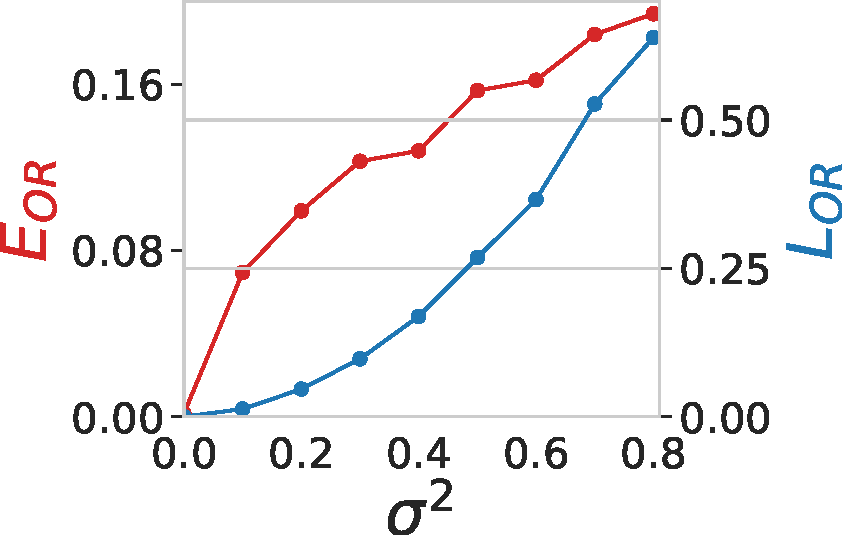
\includegraphics[width=\linewidth]{figures/5j0n_perfect_noisy_ar_aa}
            \caption{Recovering from \texttt{5j0n}.}
        \end{subfigure}
        \hfill
        \begin{subfigure}[b]{0.49\linewidth}
        \centering
            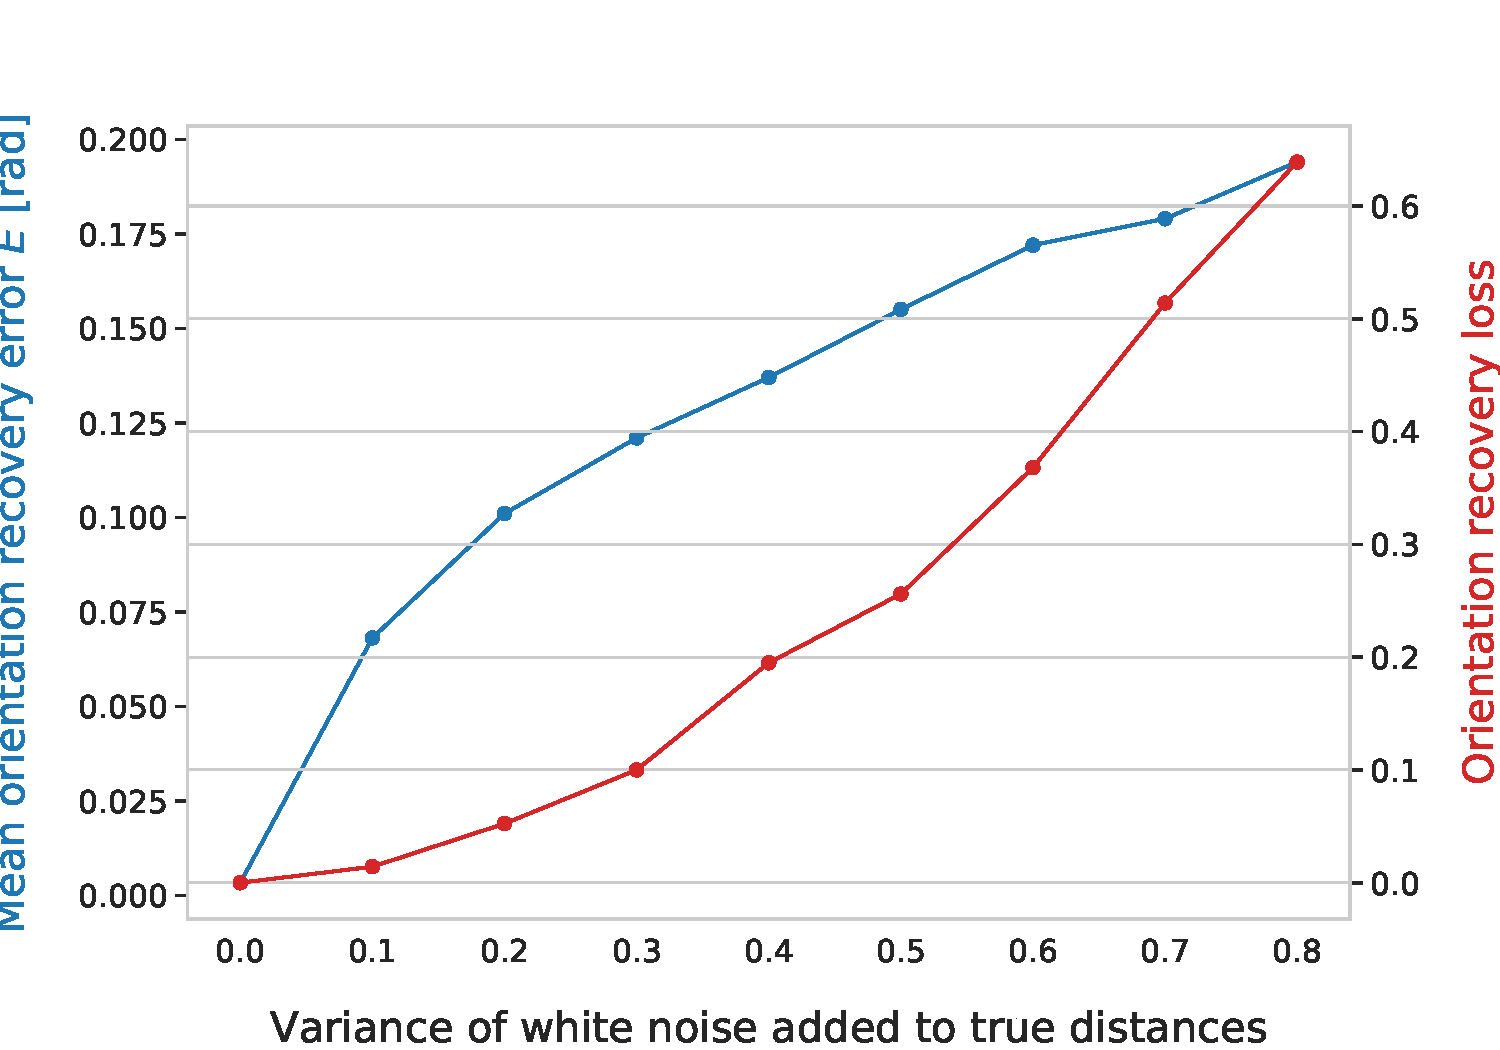
\includegraphics[width=\linewidth]{figures/5a1a_perfect_noisy_ar_aa}
            \caption{Recovering from \texttt{5a1a}.}
        \end{subfigure}
        \caption{%
            Orientation recovery from perturbed distances.
        }\label{fig:perfect-with-noise-ar-aa}
    \end{minipage}
    \hfill
    \begin{minipage}[b]{0.45\linewidth}
        \begin{subfigure}[b]{0.47\linewidth}
            \centering
            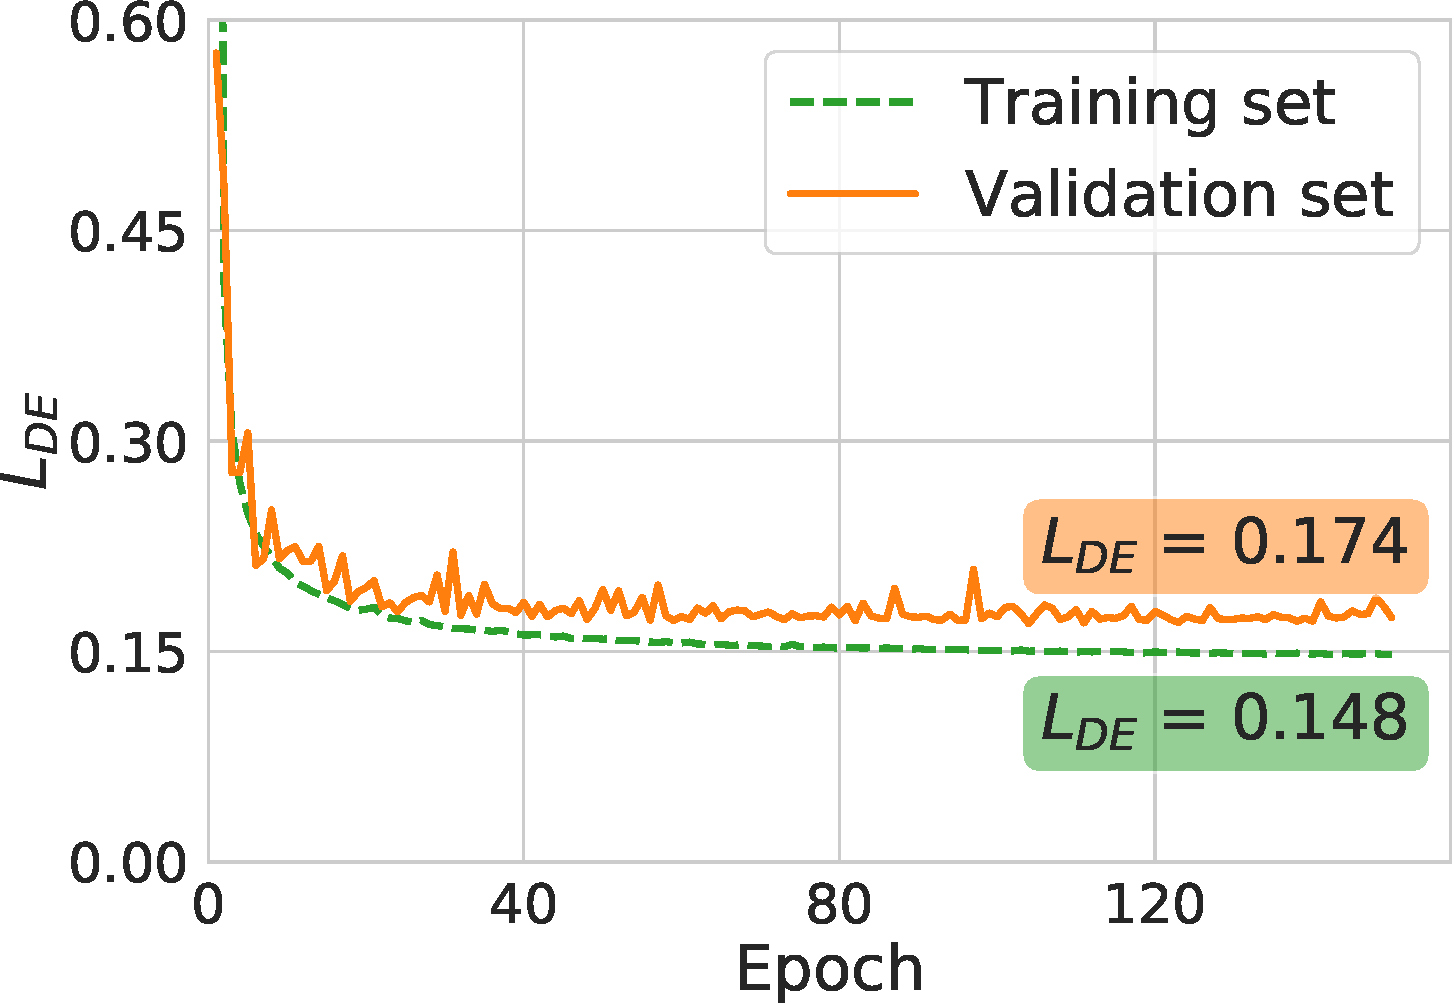
\includegraphics[width=\linewidth]{figures/de_5j0n.pdf}
            \caption{Learning from \texttt{5j0n}.\vspace{0.5em}}
        \end{subfigure}
        \hfill
        \begin{subfigure}[b]{0.47\linewidth}
            \centering
            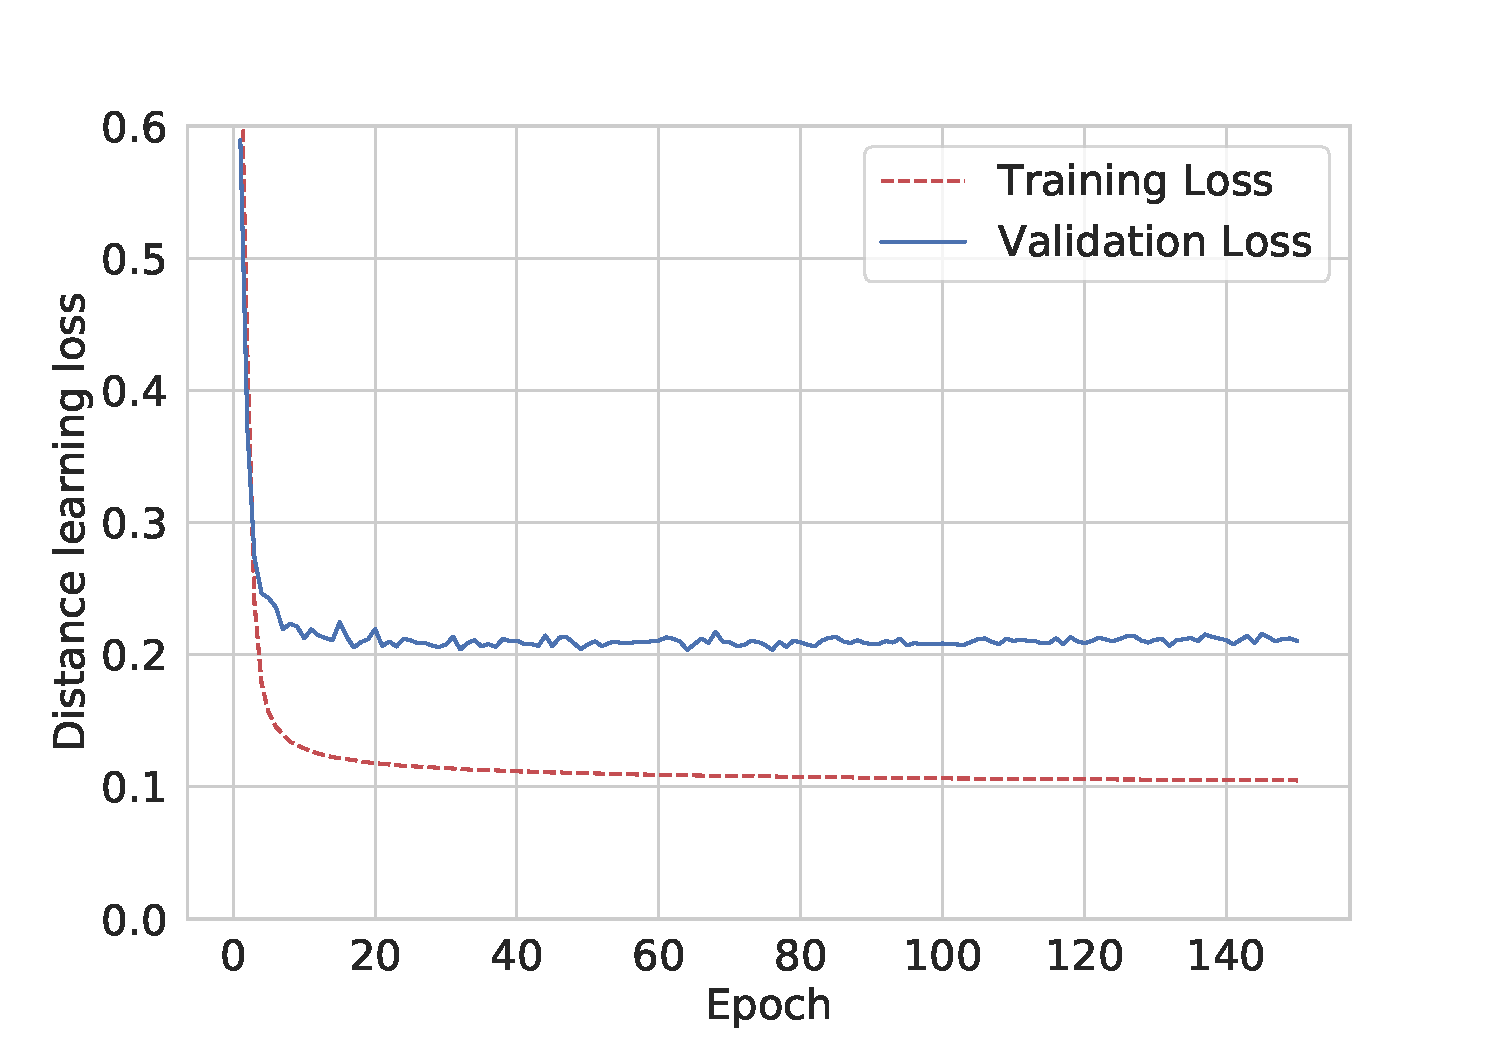
\includegraphics[width=\linewidth]{figures/de_5a1a.pdf}
            \caption{Learning from \texttt{5a1a}.\vspace{0.5em}}
    %, \; \mathbf{n} \sim \mathcal{N}(0, 16\mathbf{I})$}
        \end{subfigure}
        \\ %\vspace{1em}
        \begin{subfigure}[b]{0.47\linewidth}
            \centering
            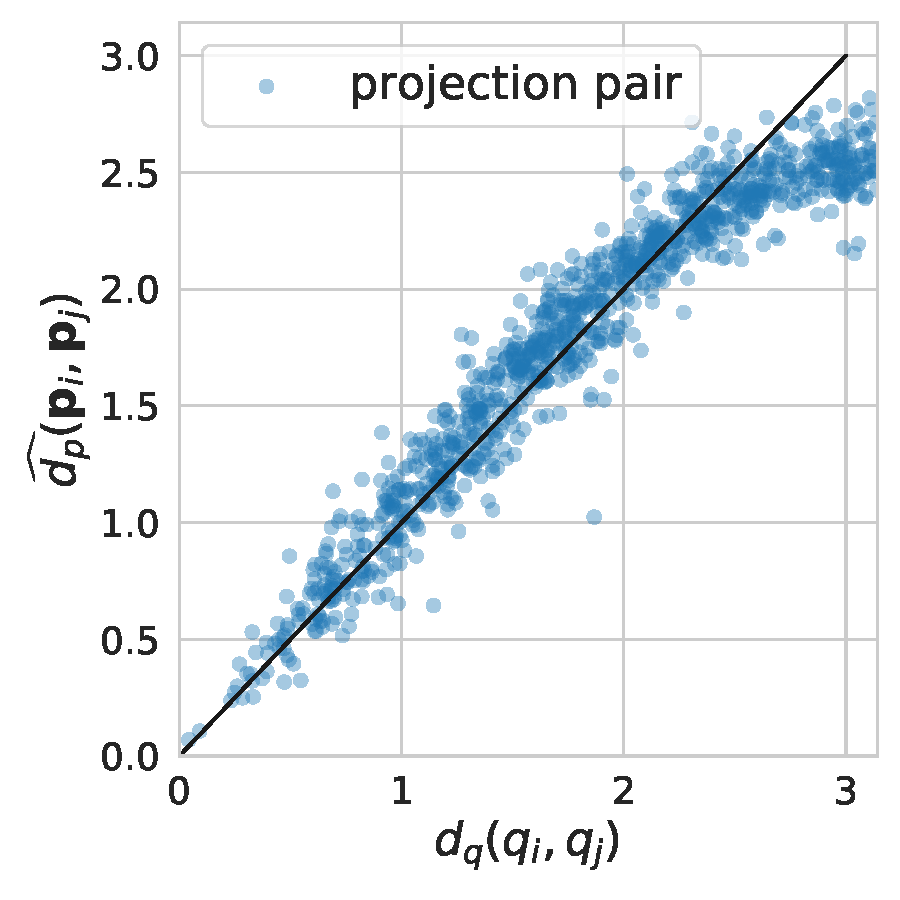
\includegraphics[width=\linewidth]{figures/dPdQ_5j0n.pdf}
            \caption{Estimating from \texttt{5j0n}.}
        \end{subfigure}
        \hfill
        \begin{subfigure}[b]{0.47\linewidth}
            \centering
            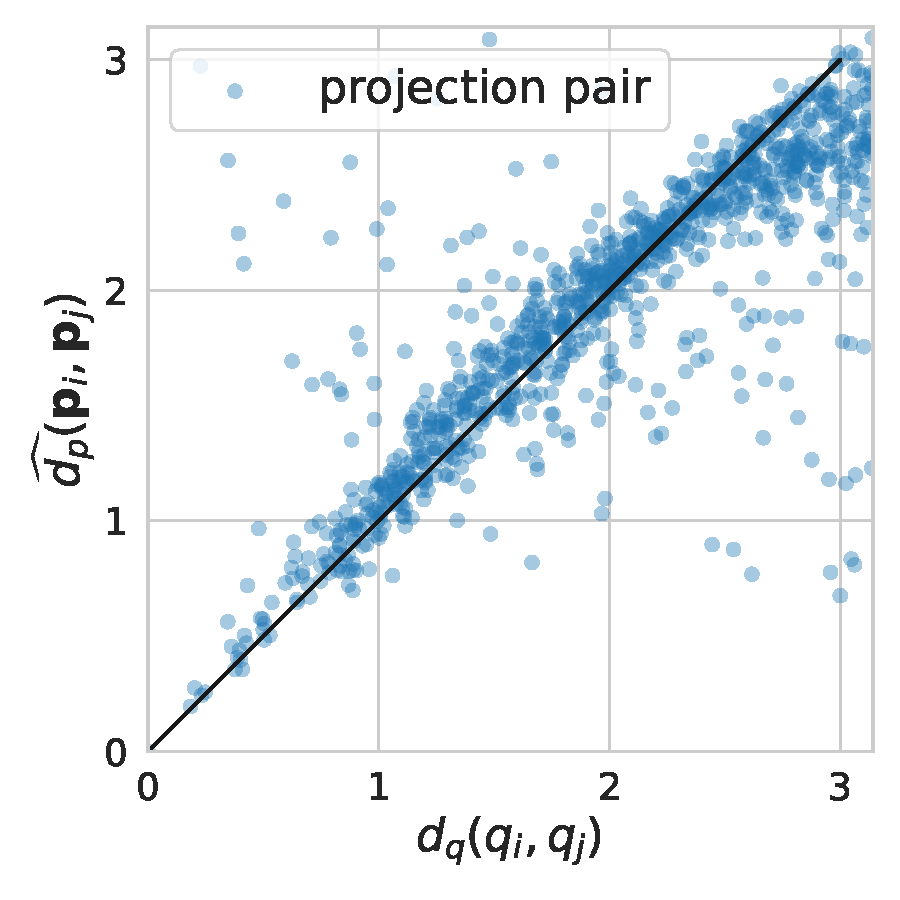
\includegraphics[width=\linewidth]{figures/dPdQ_5a1a.pdf}
            \caption{Estimating from \texttt{5a1a}.}
        \end{subfigure}
        \caption{%
            Distance learning.
            (a,b)~Convergence of the loss $L_\text{DE}$ from \eqnref{distance-learning}.
            (c,d)~Relationship between $\widehat{d_p}$ and $d_q$ on $1,000$ pairs randomly sampled from the test sets.
            \todo{y-ticks 0,1,2,3 as x-ticks.}
        }\label{fig:losses-siamese}
    \end{minipage}
\end{figure}

%%%%%%%%%%%%%%%%%%%%%%%%%%%%%%%%%%%%%%%%%%%%%%%%%%%%%%%%%%%%%%%%%%%%%%%%%%%%%%%%%%%%%%%

\subsection{Learned function for relative distance estimation }\label{sec:results:distance-estimation:learned}

%\mdeff{Story: learned distance $d_{ps}$ estimates $d_q$ with some variance but still underestimates larger distances.
%Again symmetric vs asymmetric.}

%our method could approximate
We evaluated how well our SiameseNN approximates the orientation distance $d_q$.
% ---parameterized as a SiameseNN and trained---
%s to learn a distance between projections $\widehat{d_p}(\p_i,\p_j)$
For comparison, we evaluated a baseline, the Euclidean distance $d_p(\p_i,\p_j) = \|\p_i, \p_j\|_2$, in \apxref{results:distance-estimation}.

\figref{losses-siamese}(a,b) shows how the distance learning loss converged during training.
Convergence was reached in about 50 epochs. %($50 x ? / 256$ steps).
%of the distance evolution of the training and validation losses for \texttt{5j0n} and \texttt{5a1a} are presented in and \figref{losses-siamese-sym}, respectively.
\todo{Values: $L_\text{DE} = ?$ for training/validation and \texttt{5j0n}/\texttt{5a1a}.}
While overfitting is low (the training and validation losses are close) for \texttt{5j0n}, it is larger for \texttt{5a1a}.
That's an indication that while we could train and learn a good distance on seen projections (training set), it doesn't generalize well to unseen projections (validation set).
That suggests that \texttt{5a1a} is harder than \texttt{5j0n}. \lau{Hypotheses: Some proteins have 3D density maps whose projections with close orientations are harder to distinguish from one another. Handling of symmetries could be done wrongly.}
\mdeff{Why is \texttt{5a1a} harder? Recurring theme (see 3.5).}
\mdeff{Here's an explanation by Jelena. Is it a good one? Let's discuss.}
\todo{This is most likely due to the symmetry of the protein (even though a quarter-sphere coverage was used.
%Indeed, its synthetic dataset may still contain pairs of projections that share the same $d_p$, yet differ in their $d_q$.
This  advocates for restricting to non-overlapping areas of $\SO(3)$ the sampling of the orientations used to generate the training dataset.
The latter would then only contain projection pairs with a linear $(d_q,d_p)$ relationship, which should ensure a successful training of the network.}
%\mdeff{I don't get this explanation. Do you mean that \texttt{5a1a} might have other symmetries than D2?}

\figref{losses-siamese}(c,d) shows the relation between the estimated distance $\widehat{d_p}$ and true distance $d_q$.
As expected, distances are better estimated for \texttt{5j0n} than \texttt{5a1a}.
While our learned distance function is a much better estimator than the Euclidean distance (compare \figref{losses-siamese}(c,d) with \figref{euclidean-not-robust}), they share one characteristic: both plateau and underestimate larger distances.
Though the issue is much less severe that with Euclidean distance.
\todo{Hypotheses: Because the true distances are upper-bounded by $\pi$? Training? Fixing a bit by sampling distances uniformly.}
Resolving this issue would ...
An alternative is to discard the larger distances and only rely on the estimation of local / short distances.
That would however require a force/loss/counter-balancing in \eqnref{orientation-recovery} to spread the orientations and prevent them to collapse to a single point.

% proxy distance
These results confirm that a SiameseNN is able to estimate differences in orientations from projections alone.
%Moreover, it clearly outperformed the Euclidean distance at doing so.
These preliminary results are encouraging; indeed, much has yet to be gained from improving upon the rather primitive SiameseNN architecture we are currently using.
Then train on more data (more pairs, data augmentation from imaging model \eqnref{imaging-model}, more proteins).
% Insist because that's a recurring theme of the paper.
Those will especially help when the task is more difficult, as for \texttt{5a1a}.
More data required to close the gap on \texttt{5a1a}, more powerful SiameseNN to push the losses down on both.
% Recurring theme.

%%%%%%%%%%%%%%%%%%%%%%%%%%%%%%%%%%%%%%%%%%%%%%%%%%%%%%%%%%%%%%%%%%%%%%%%%%%%%%%%%%%%%%%

\subsection{Sensitivity of distance learning to perturbations in the projections}\label{sec:results:distance-estimation:sensitivity}
%\subsection{Generalization of distance learning}
%\subsection{Generalizability/Abstractability of distance learning}

%\mdeff{Shall we use ``noiseless projections'' or ``clean projections''?} \lau{Noiseless if space is not an issue.}

%\mdeff{Story: learned distance is minimally sensible to perturbations (additive noise, translation, PSF) because we can train it to ignore irrelevant information.
%Thanks again to good model of cryo-EM imaging.}
%\mdeff{Better word? (perturbations, corruptions, quality, non-ideal)}

% Intro and shift.
We desire to estimate distances that are invariant to perturbations in the projections---specified in~\eqnref{imaging-model}.
As discussed in \secref{method:distance-learning}, the convolutional architecture of the SiameseNN should be shift invariant.
\figref{results:distance-estimation:shift} indeed shows that learning distances (and hence recovering orientations) is insensible to shifts in projections.

% Noise.
As we cannot---or do not (yet) know how to---build noise invariance into the architecture, we trained the SiameseNN on noisy datasets and evaluated whether it could learn to ignore noise as being irrelevant information.
% brute force vs principled engineering
\figref{results:distance-estimation:noise} shows $E_\text{OR} \approx 0.16$ radians ($\approx 9\degree$) for noiseless projections and $E_\text{OR} \approx 0.42$ radians ($\approx 24\degree$) for a more realistic noise variance of $\sigma^2=16$.
%\mdeff{How good is that?}\banjac{To be discussed tomorrow}\lau{Reasonable first guess, room for improvement.}
While a naive distance function (like an Euclidean distance) would be tremendously sensitive to noise, the SiameseNN mostly learned to discard it.
Moreover, overfitting (i.e., the growing gap between the validation and training losses) indicates that more training data will further decrease the SiameseNN's sensitivity to noise.
While the results are good, there is also room for improvement.

% PSF and conclusion.
We didn't evaluate sensitivity to the PSF but expect a similar behavior.
%While we would ideally want the NN architecture to be engineered to ignore irrelevant information, that is not always possible.
%We know how to do it for shifts, not noise or PSF.

We observe that the estimation of more accurate distances (a smaller $L_\text{DE}$) leads to the recovery of more accurate orientations (a smaller $L_\text{OR}$ and $E_\text{OR}$).
Moreover, we observe again (\secref{results:orientation-recovery:sensitivity}) that an higher recovery loss $L_\text{OR}$ induces an higher error $E_\text{OR}$.

%\subsection{Estimating distances on unseen proteins}

As the SiameseNN will ultimately be trained on known proteins and used to estimate distances on unknown proteins to be imaged,
%we also desire our learned distance function to generalize/transfer across density maps $\x$.
we also desire our learned distance function to generalize to unseen proteins.
The distance function $\widehat{d_p}$ must abstract the protein (in the same way it must abstract shifts, noise, or PSFs to generalize to unseen projections).
We attempted to recover the orientations of noiseless projections from \texttt{5j0n} while we had trained the SiameseNN on noiseless projections of four other proteins (\texttt{5nvu}~\cite{5nvu_pdb}, \texttt{5nvs}~\cite{5nvs_pdb}, \texttt{6mem}~\cite{6mem_pdb}, \texttt{6o1o}~\cite{6o1o_pdb} \todo{should be the same ``kind'' of refs as the ones used in 3.1 for \texttt{5j0n} and \texttt{5a1a}}, which have the same type of symmetry as \texttt{5j0n}).
In this experiment, we generated $1,000$ projections per protein.
Four proteins were used in the training and validation set to ensure the robustness to the unseen protein \texttt{5j0n} used in the testing set.
The number of projections in every set is the same as in \tabref{dataset}.
We obtained a recovery loss of $L_\text{OR} = 0.0352$ \mdeff{Could we also have $E_\text{OR}$? It's easier to understand and compare.}\banjac{I fully agree, however, I already mentioned that I wasn't able to align the orientations even though the $L_\text{OR}$ was very good. Looking at the estimation and GT in rotation space, it is visible we have some kind of transformation between these two (transformation similar to one we found the flip is causing, but it is not the flip)},
\mdeff{Right, thanks for explaining again. We should probably talk about that issue somewhere. An Appendix? Do we have examples when it worked and when it didn't?}\banjac{coming soon}
% Jelena: Angle recovery is good but it is unable to align. Probably missing something as expected as a flip discovered at the beginning of the project.
to be compared with $L_\text{OR} \approx 0.11$ when the SiameseNN was trained on \texttt{5j0n} alone.
While performance is somewhat degraded, we conclude that it is possible to use a learned distance function on unseen proteins.

\begin{figure}[ht!]
    \centering
    \begin{subfigure}[t]{0.47\linewidth}
        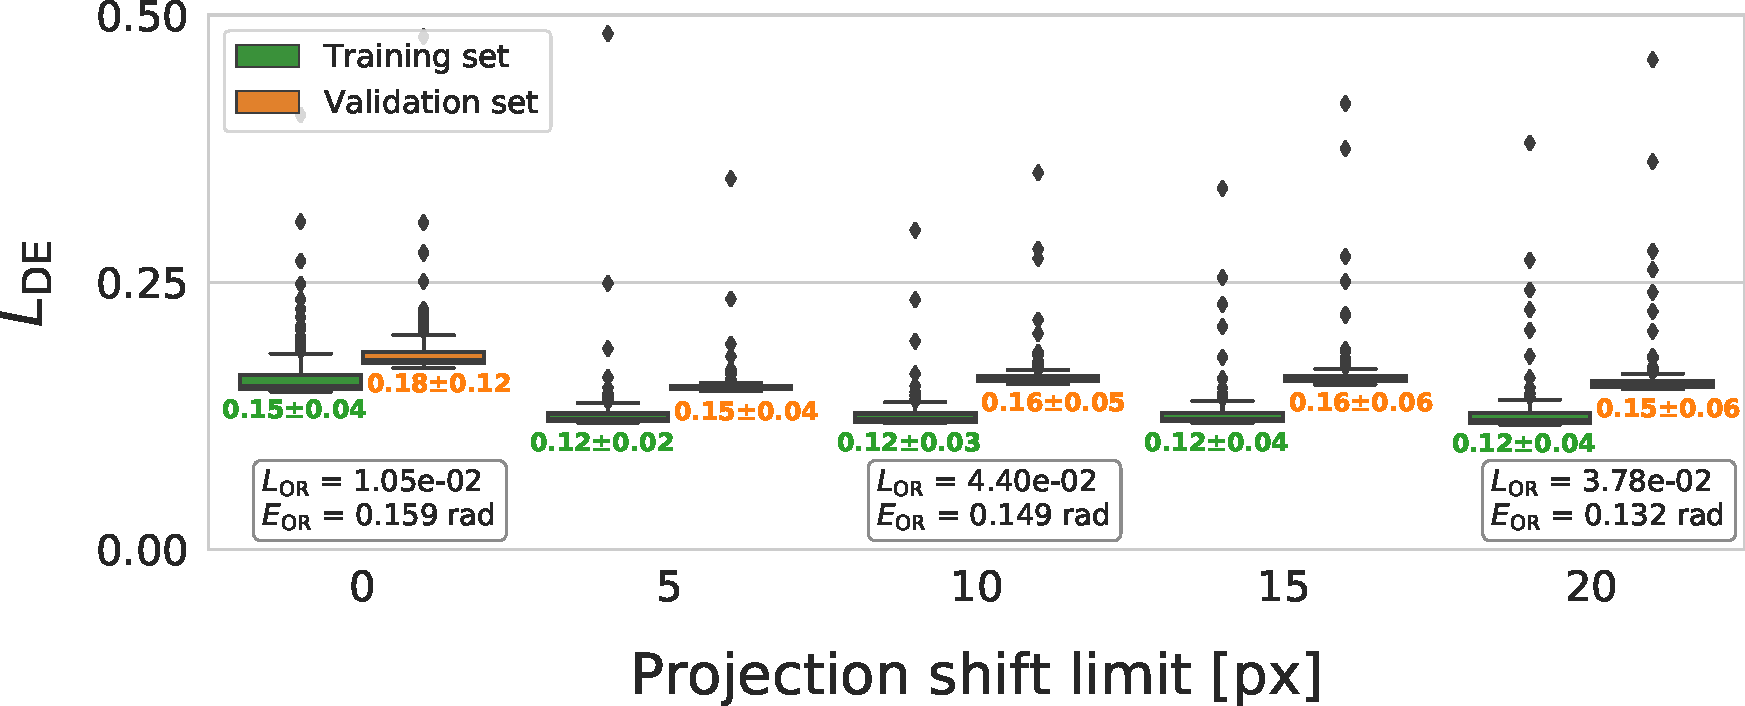
\includegraphics[width=\linewidth]{figures/de_translation_nums}
        \caption{%
            Learning from shifted projections $\{ \mathbf{S}_{\mathbf{t}_i} \mathbf{P}_{\bth_i} \mathbf{x} \}$, with translations $t_{i_1}$ and $t_{i_2}$ sampled from a triangular distribution with mean 0 and of increasing limits.
            Learning is not harder as projections get shifted farther, because shift invariance is built into the convolutional architecture of $\mathcal{G}_w$.
    }\label{fig:results:distance-estimation:shift}
    \end{subfigure}
    \hfill
    \begin{subfigure}[t]{0.47\linewidth}
        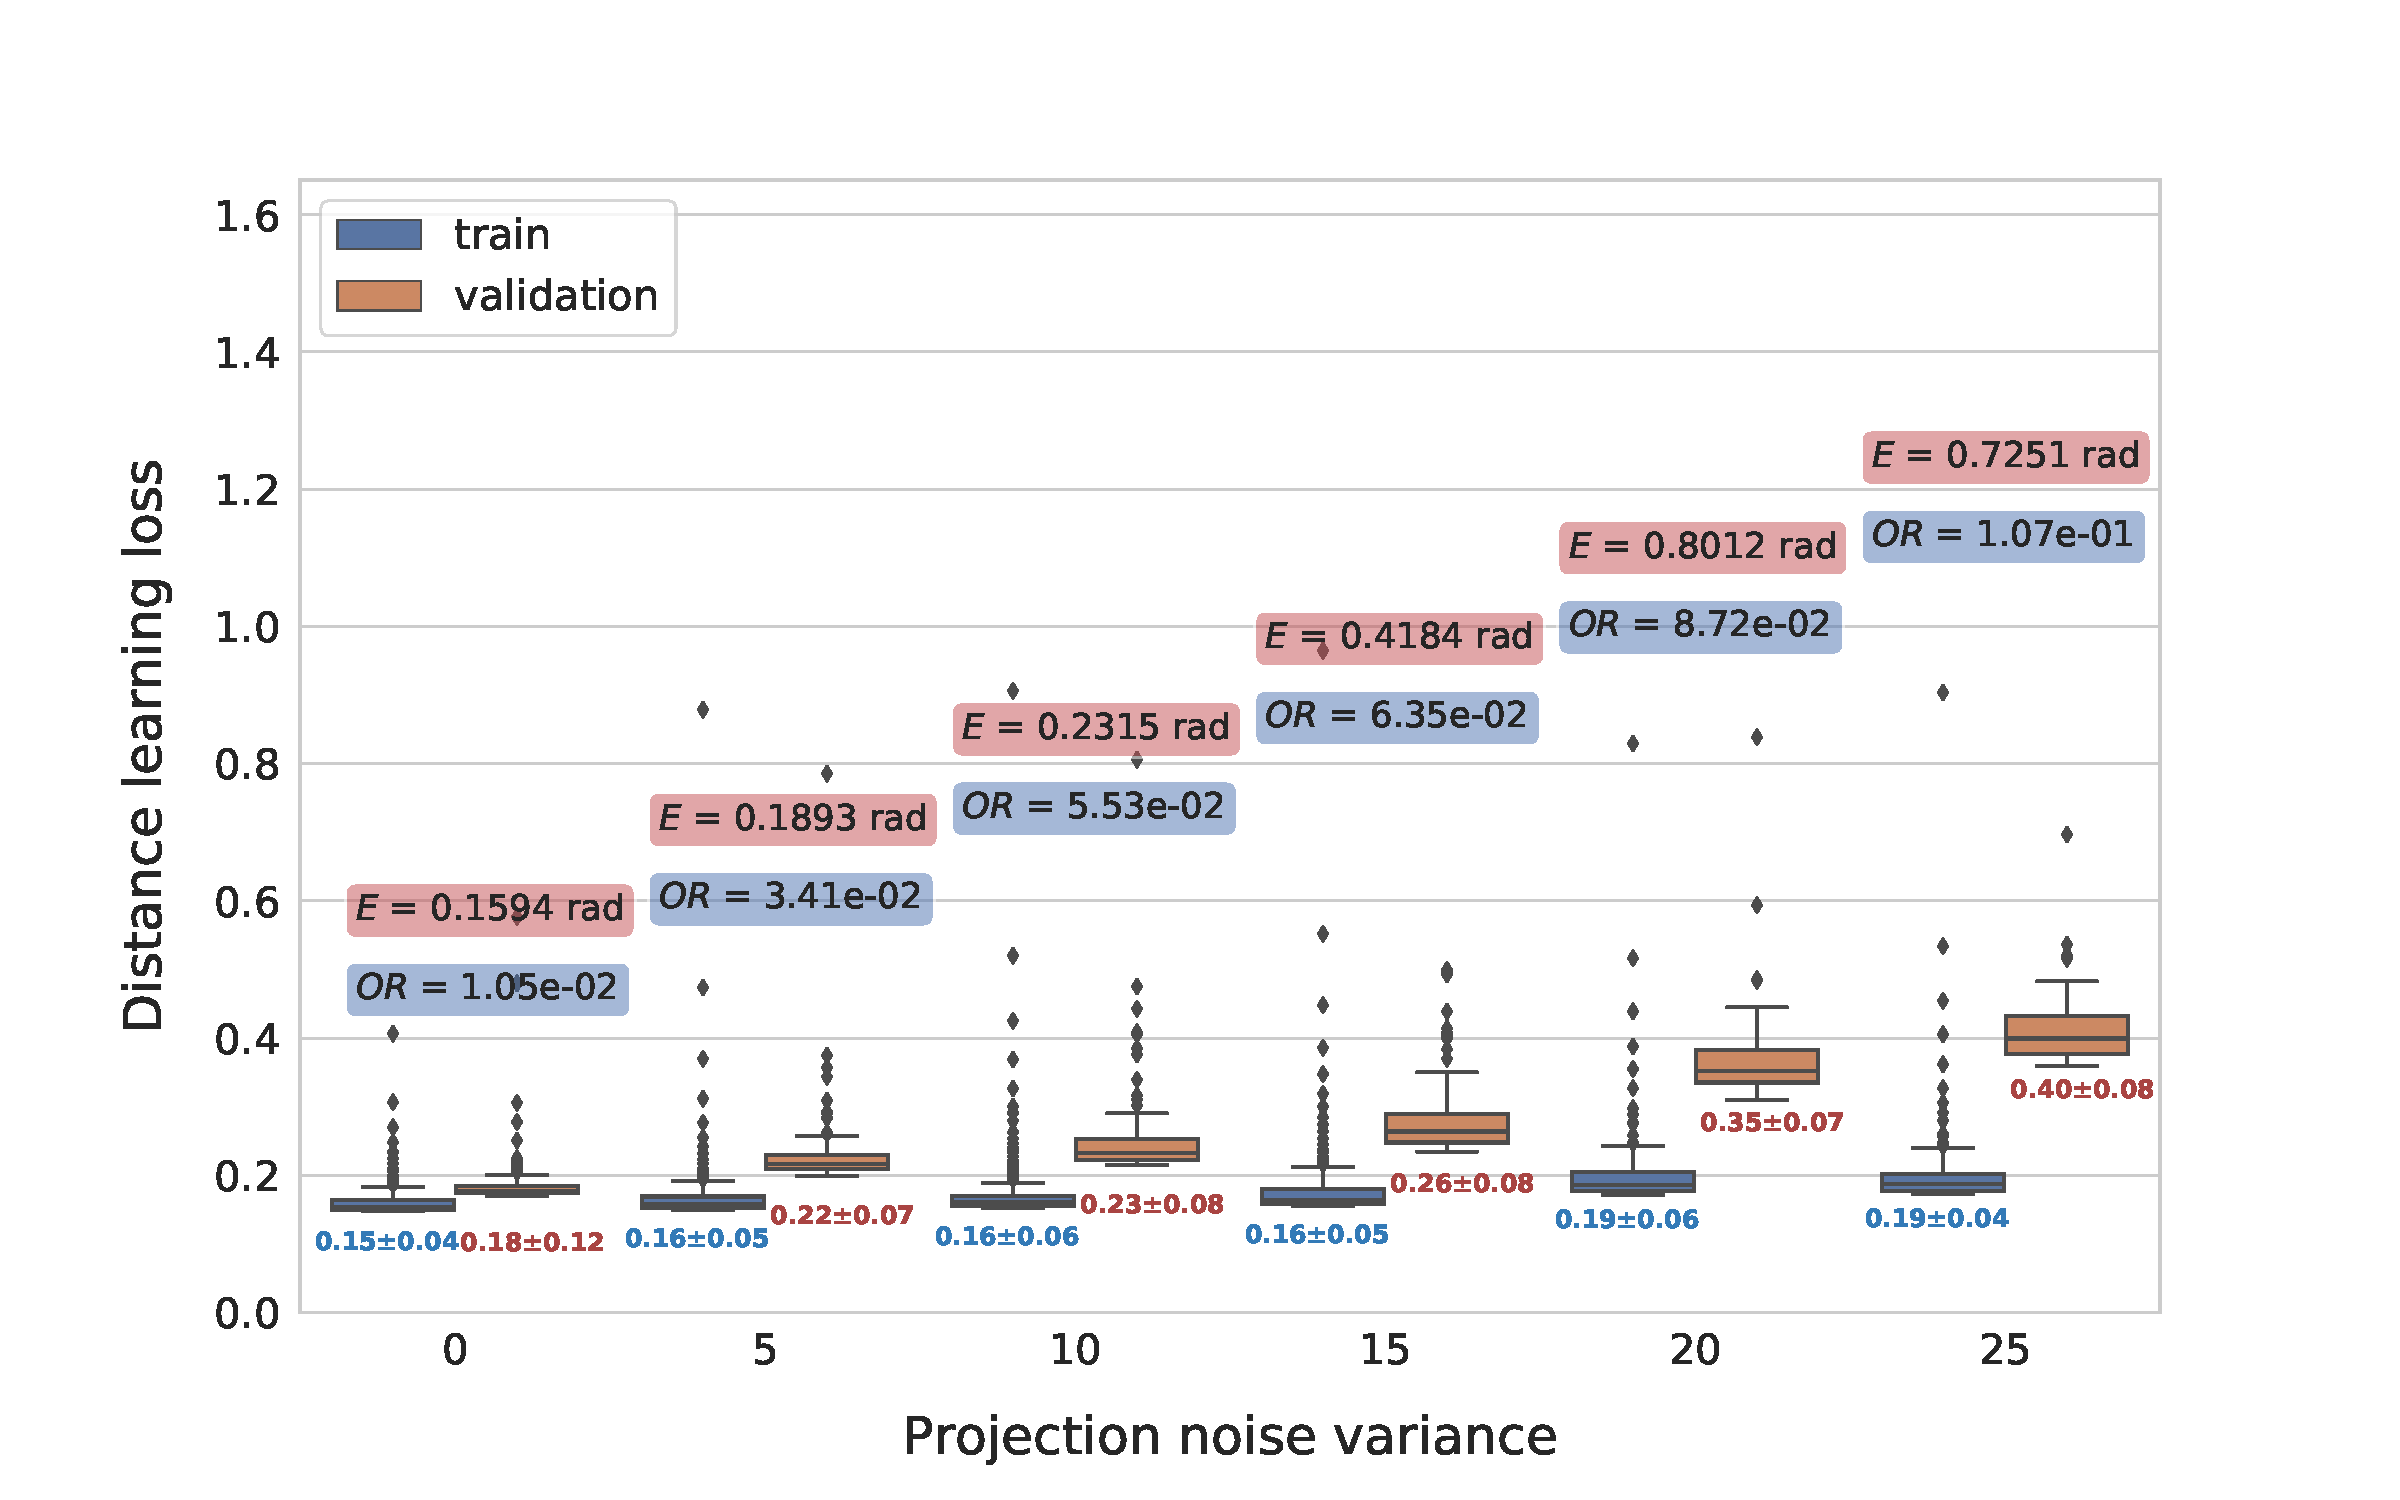
\includegraphics[width=\linewidth]{figures/de_noises_nums}
        \caption{%
            Learning from noisy projections $\{ \mathbf{P}_{\bth_i} \mathbf{x} + \mathbf{n} \}$, with white noise $\mathbf{n} \sim \mathcal{N}(0, \sigma^2\mathbf{I})$ of increasing variance $\sigma^2$.
            Learning is harder as projections get noisier, because noise invariance is not built into the architecture of $\mathcal{G}_w$.
        }\label{fig:results:distance-estimation:noise}
    \end{subfigure}
    \caption{%
        Sensitivity of distance learning to perturbations in the projections of \texttt{5j0n}.
        The box plots show the distance learning loss $L_\text{DE}$ per epoch \eqnref{distance-learning} on the training (blue) and validation (red) sets.
        %\mdeff{Numbers are per pair or per batch of 256 pairs?}
        Boxes show the orientation recovery loss $L_\text{OR}$ \eqnref{orientation-recovery} and error $E_\text{OR}$ \eqnref{orientation-recovery-error}.
        %\mdeff{It's confusing that red and blue are used for both train vs validation and $E_\text{OR}$ vs $L_\text{OR}$. I don't think we need colors for $E_\text{OR}$ and $L_\text{OR}$. They could both be in the same black box.}
        %\todo{Legend consistency: train -> training set, validation -> validation set.}
        %\todo{Add $L_\text{DE}$ to the y-axis legend.}
        %\todo{Add $\sigma^2$ to the x-axis legend of (b).}
    }
\end{figure}

%%%%%%%%%%%%%%%%%%%%%%%%%%%%%%%%%%%%%%%%%%%%%%%%%%%%%%%%%%%%%%%%%%%%%%%%%%%%%%%%%%%%%%%

\subsection{Orientation recovery and density reconstruction from estimated distances}\label{sec:results:orientation-recovery:reconstruction}
%\subsection{Density reconstruction from recovered orientations}

\todo{
\begin{itemize}
    \item \mdeff{Should we call it Density reconstruction from recovered orientations?}\banjac{Density sounds very general to me, 3d protein reconstruction, protein electron density reconstruction?  Or even Complete machine learning pipeline}
    %\item Make the plots in Figures~\ref{fig:5j0n-noise0-orientation-recovery},~\ref{fig:5j0n-noise16-orientation-recovery}, and~\ref{fig:5a1a-noise0-orientation-recovery} flatter and remove \texttt{width=linewidth} (which deforms the figure).
    %\item Add $L_\text{OR}=...$ and $E_\text{OR}=...$ in the boxes of Figures~\ref{fig:5j0n-noise0-orientation-recovery},~\ref{fig:5j0n-noise16-orientation-recovery}, and~\ref{fig:5a1a-noise0-orientation-recovery}.
    \item Would be nice to know $L_\text{DE}$ for the three cases. \banjac{On the test set?}
    %\item ``With total of $1,650$ projections in the test dataset, we were able to reconstruct the protein.'' \mdeff{But \tabref{dataset} says 838 for test. Was it validation data?} \banjac{Great notice!! The table was wrong, I fixed it. In the code I was printing in different order so I mixed it.}
    %\item \mdeff{Training set for distance learning and validation/test set for orientation recovery should have been made clear in 3.1.} \banjac{Actually, train and validation sets are used in distance learning, and test set was only used for dPdQ plot, orientation recovery (and alignment)}
\end{itemize}
}

As a proof-of-concept, we attempted to solve the inverse problem posed by \eqnref{imaging-model}.
We reconstructed density maps $\widehat{\x}$ from sets of projections $\{ \p_i \}$ and their orientations $\{ \widehat{q_i} \}$ as recovered by our method.
%We ran the full pipeline---distance estimation, orientation recovery, and protein reconstruction---to validate our method.
%The orientation recovery from estimated distances represents a full pipeline needed to reconstruct the protein from a given set of projections.
Note that we only trained the SiameseNN \eqnref{distance-learning} on projections from the protein (and noise level) we attempted to reconstruct from.
For best performance, it should be trained on multiple proteins, levels of noise, PSFs, etc.

\lau{Smooth this paragraph:}To understand the effect of miss-recovered orientations, we reconstructed the density maps from both the recovered orientations $\{ \widehat{q_i} \}$ and the true orientations $\{ q_i \}$ along which the projections $\{ \p_i \}$ were acquired.
The density maps were reconstructed by the ASTRA toolbox.
\todo{Using the ASTRA toolbox, we generated orientation vectors based on angles which we fed into projection 3D geometry in ASTRA.}
\todo{Make clearer. Are there enough details?}
\mdeff{Laurène, could you write something about how ASTRA is a naive reconstruction method (compared to the SOTA discussed in the intro), and that we did it only to get a crude idea? Or something along those lines. ;)} \lau{Not naïve actually, just direct hence less robust. I think it's a good idea to write this, i.e. that the quality of reconstruction is likely to improve with a more robust algorithm, but I'm wondering if we should not put that in the discussion/conclusion.}
For an unknown reason, we had to align the recovered orientations with \eqnref{orientation-recovery-error} before feeding them to ASTRA.
\todo{More details. What happened otherwise? We want to say it's an ASTRA issue not something with our method.} \lau{Yeah but I wouldn't blame ASTRA at all, it's dangerous territory. There is just an engineering problem we haven't been able to solve, let's not blame well-know, widely-used existing packages out there if possible.}

\begin{figure}[t]
    \centering
    \begin{subfigure}[b]{0.44\linewidth}
        \centering
        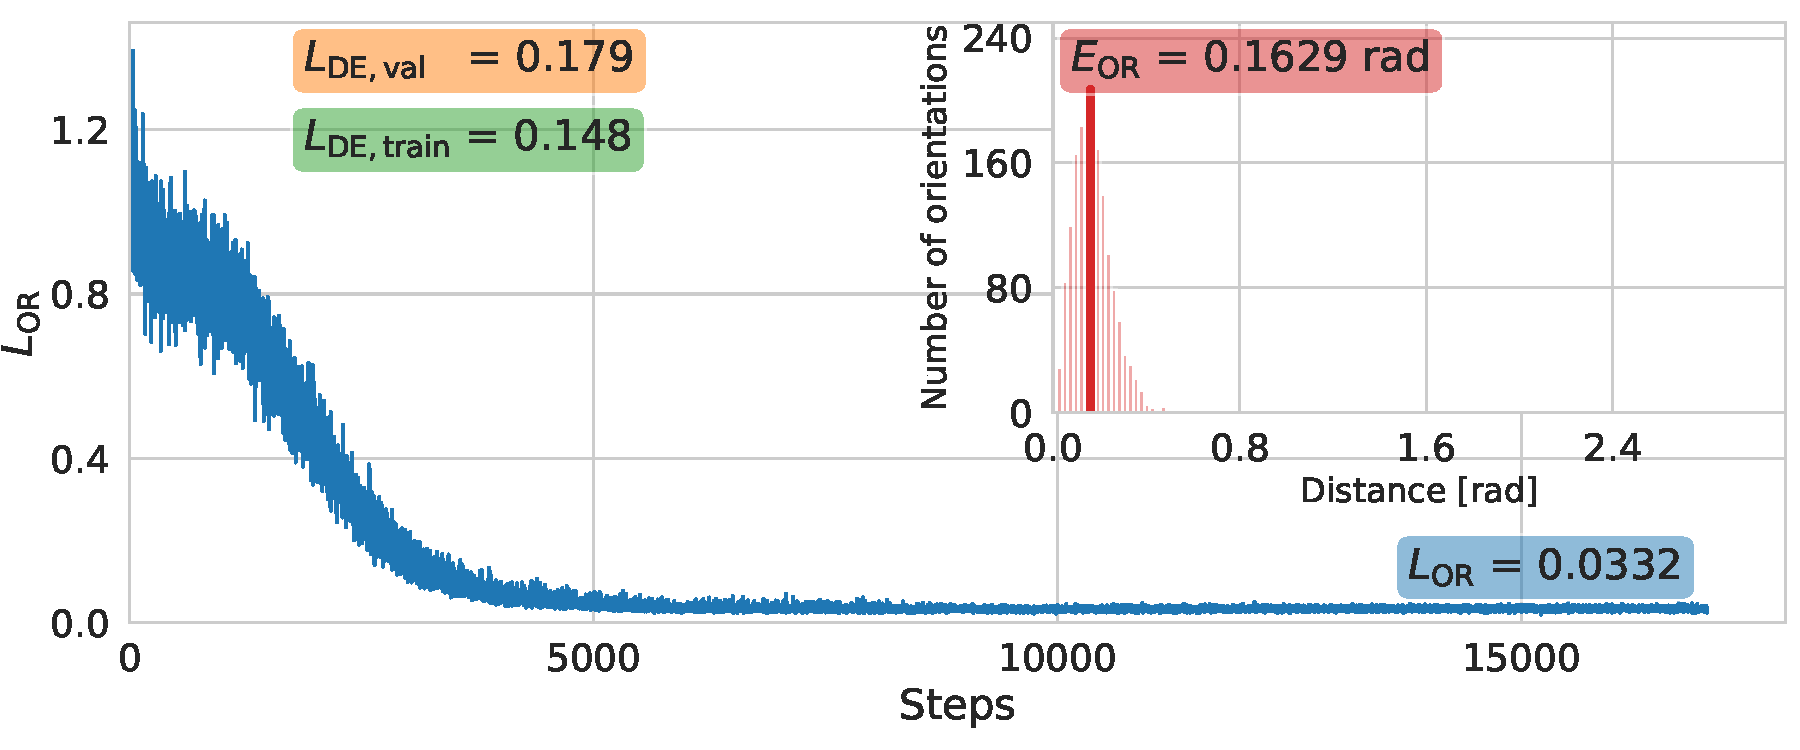
\includegraphics[height=8em]{figures/5j0n_noise0_ar_aa}
        \caption{Recovered $\{ \widehat{q_i} \}$ from noiseless \texttt{5j0n} projections $\{ \p_i \}$.
        %$\{ \p_i = \mathbf{P}_{\bth_i} \x \}$, $\x$ from \texttt{5j0n}.
        }%
        \label{fig:5j0n-noise0-orientation-recovery}
    \end{subfigure}
    \hfill
    \begin{subfigure}[b]{0.26\linewidth}
        \centering
        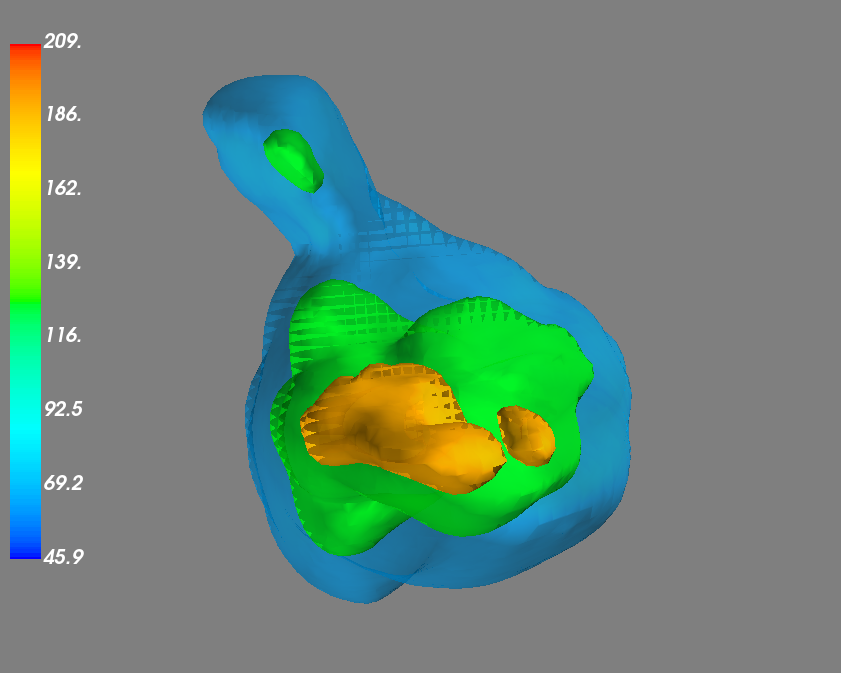
\includegraphics[height=8em]{figures/5j0n_reconstruction_noise0}
        \caption{Reconstructed $\widehat{\x}$ from $\{ \p_i, \widehat{q_i} \}$.}%
        \label{fig:5j0n-noise0-reconstruction-recovered}
    \end{subfigure}
    \hfill
    \begin{subfigure}[b]{0.26\linewidth}
        \centering
        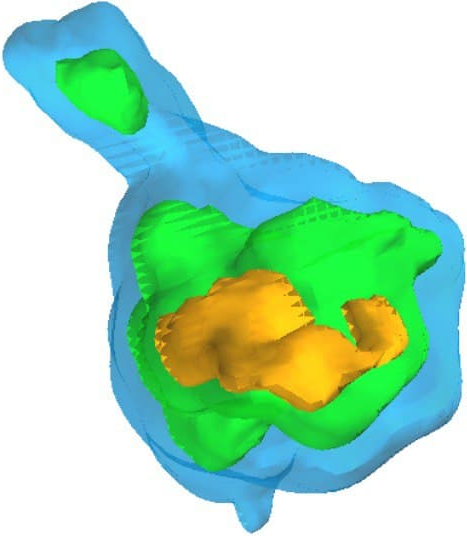
\includegraphics[height=8em]{figures/5j0n_reconstruction_GT}
        \caption{Reconstructed $\widehat{\x}$ from $\{ \p_i, q_i \}$.}%
        \label{fig:5j0n-noise0-reconstruction-true}
    \end{subfigure}
    \\ \vspace{1em}
    \begin{subfigure}[b]{0.44\linewidth}
        \centering
        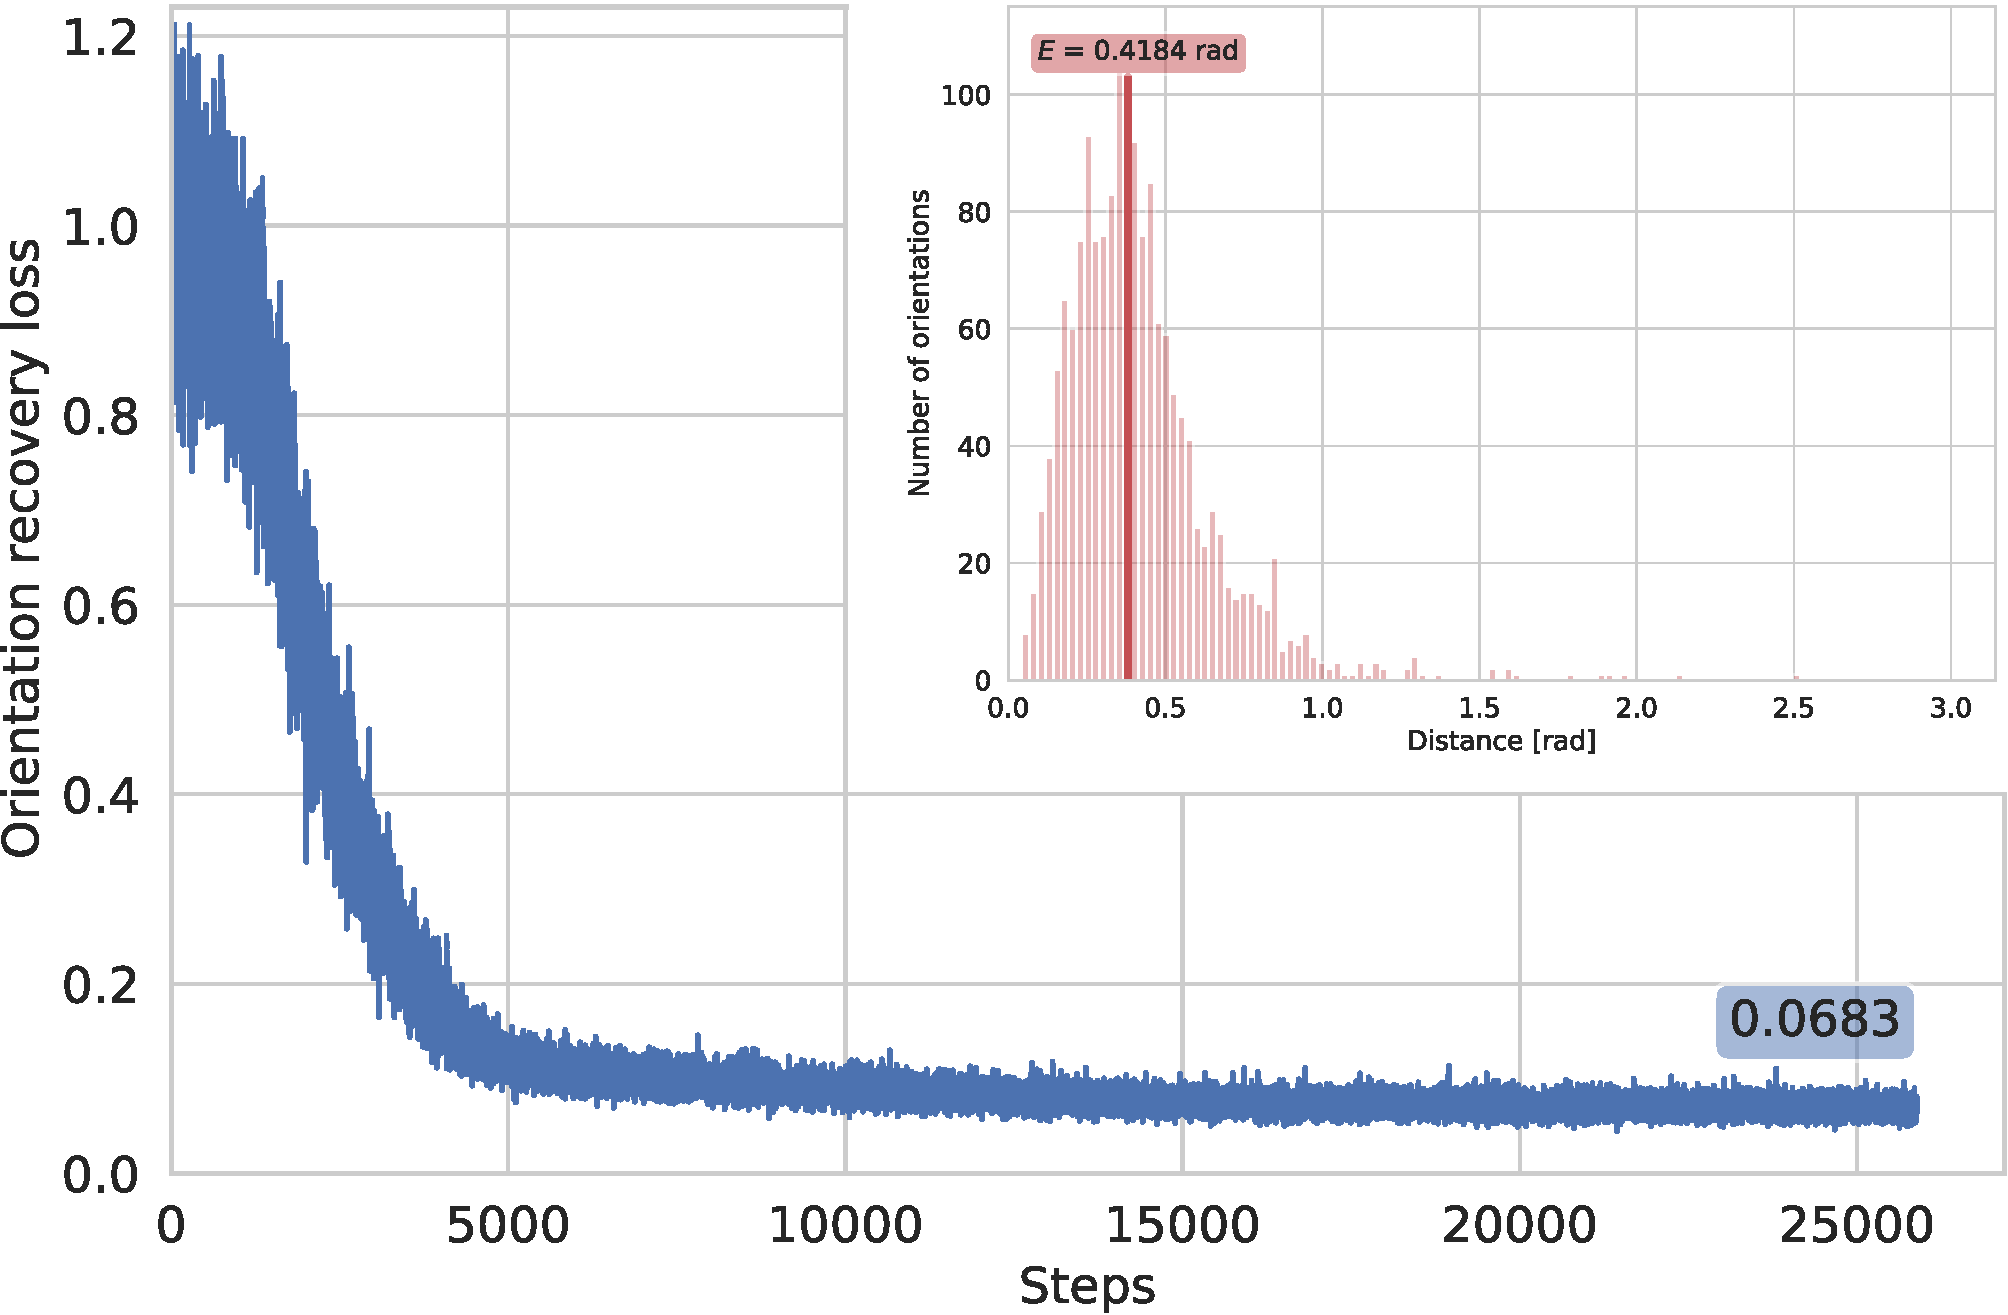
\includegraphics[height=8em]{figures/5j0n_noise16_ar_aa}
        \caption{Recovered $\{ \widehat{q_i} \}$ from noisy \texttt{5j0n} projections $\{ \p_i \}$.
        %$\{ \p_i = \mathbf{P}_{\bth_i} \x + \mathbf{n} \}$, $\x$ from \texttt{5j0n}.
        }%
        \label{fig:5j0n-noise16-orientation-recovery}
    \end{subfigure}
    \hfill
    \begin{subfigure}[b]{0.26\linewidth}
        \centering
        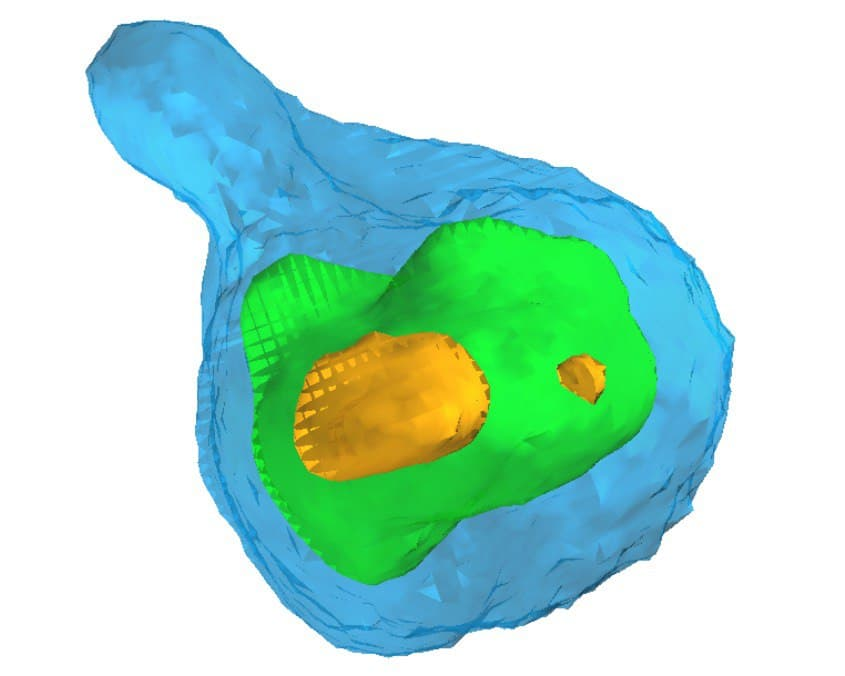
\includegraphics[height=8em]{figures/5j0n_reconstruction_noise16}
        \caption{Reconstructed $\widehat{\x}$ from $\{ \p_i, \widehat{q_i} \}$.}%
        \label{fig:5j0n-noise16-reconstruction-recovered}
    \end{subfigure}
    \hfill
    \begin{subfigure}[b]{0.26\linewidth}
        \centering
        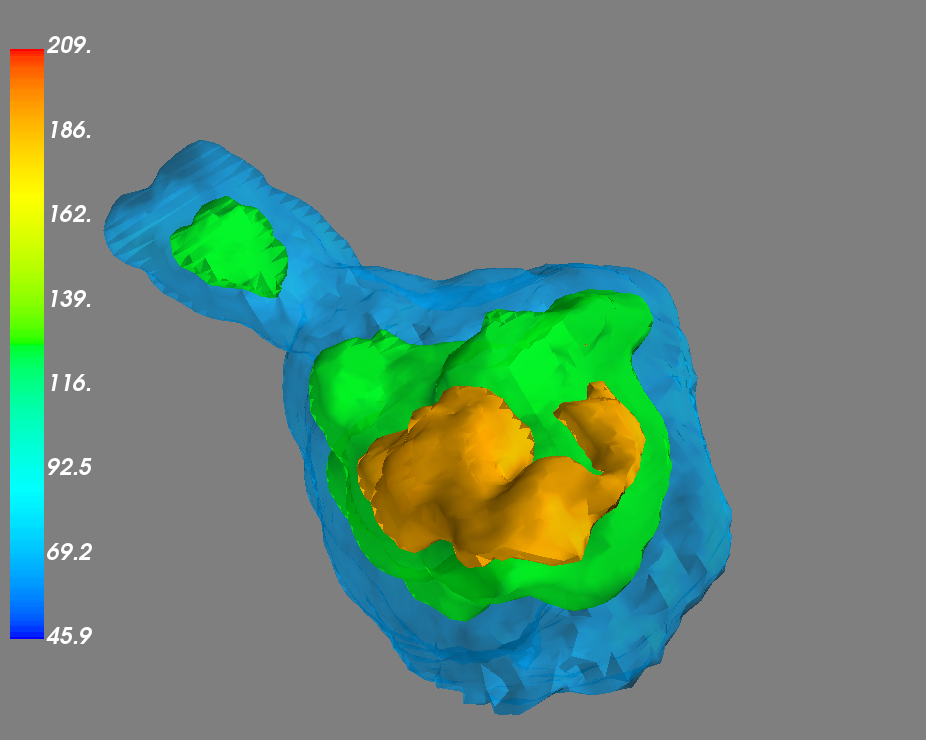
\includegraphics[height=8em]{figures/5j0n_reconstruction_GT_noise16}
        \caption{Reconstructed $\widehat{\x}$ from $\{ \p_i, q_i \}$.}%
        \label{fig:5j0n-noise16-reconstruction-true}
    \end{subfigure}
    \\ \vspace{1em}
    \begin{subfigure}[b]{0.44\linewidth}
        \centering
        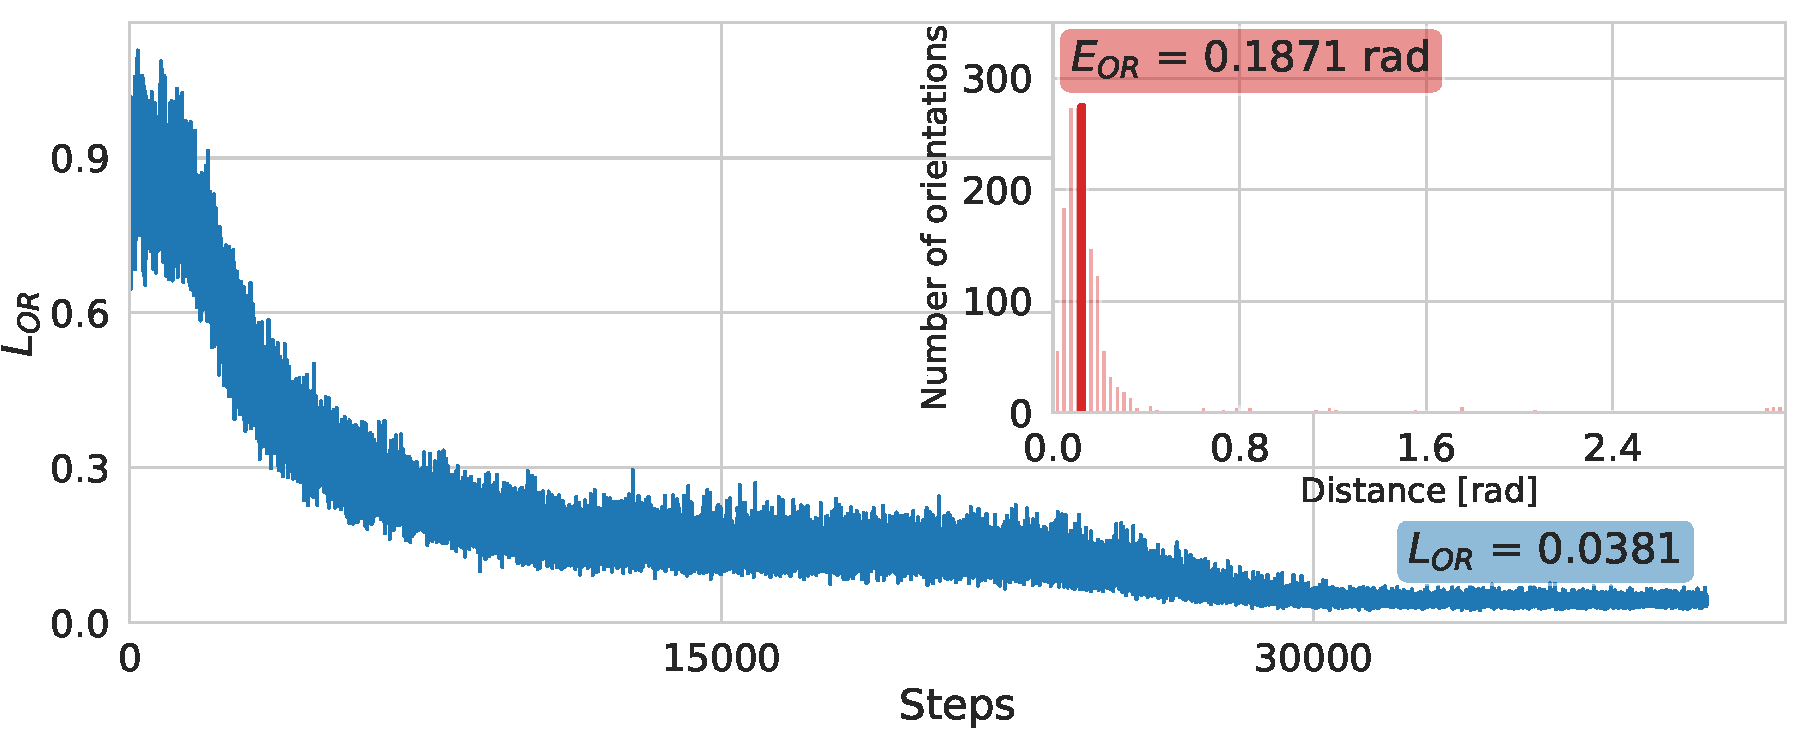
\includegraphics[height=8em]{figures/5a1a_noise0_ar_aa}
        \caption{Recovered $\{ \widehat{q_i} \}$ from noiseless \texttt{5a1a} projections $\{ \p_i \}$.
        %$\{ \p_i = \mathbf{P}_{\bth_i} \x \}$, $\x$ from \texttt{5a1a}.
        }%
        \label{fig:5a1a-noise0-orientation-recovery}
    \end{subfigure}
    \hfill
    \begin{subfigure}[b]{0.26\linewidth}
        \centering
        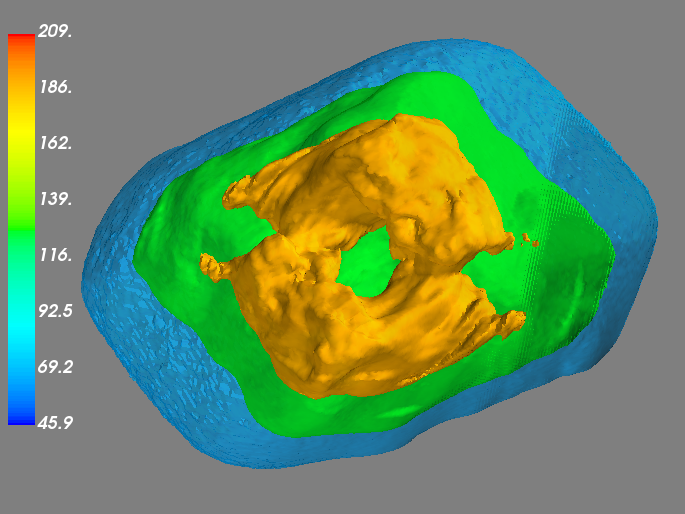
\includegraphics[height=8em]{figures/5a1a_aligned}
        \caption{Reconstructed $\widehat{\x}$ from $\{ \p_i, \widehat{q_i} \}$.}%
        \label{fig:5a1a-noise0-reconstruction-recovered}
    \end{subfigure}
    \hfill
    \begin{subfigure}[b]{0.26\linewidth}
        \centering
        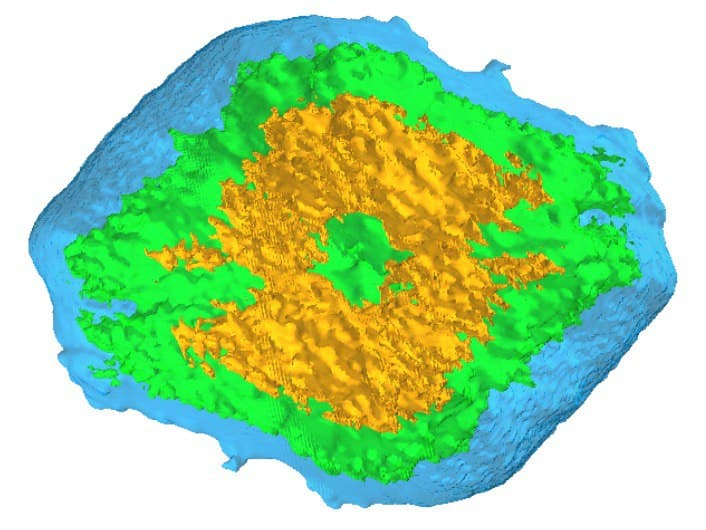
\includegraphics[height=8em]{figures/5a1a_ground_truth}
        \caption{Reconstructed $\widehat{\x}$ from $\{ \p_i, q_i \}$.}%
        \label{fig:5a1a-noise0-reconstruction-true}
    \end{subfigure}
    \caption{%
        Orientation recovery and density reconstruction from estimated distances.
        The first column~(a,d,g) shows orientation recovery:
        The blue curve shows the evolution of the recovery loss until convergence, with the minimum $L_\text{OR}$ \eqnref{orientation-recovery} highlighted.
        The red histogram shows the errors in the recovered orientations $\{d_q(q_i, \mathbf{T}\widehat{q_i})\}$, with the mean $E_\text{OR}$ \eqnref{orientation-recovery-error} highlighted.
    The second and third columns show density maps $\widehat{\x}$ reconstructed from projections $\{ \p_i \}$, and recovered orientations $\{ \widehat{q_i} \}$~(b,e,h) or true orientations $\{ q_i \}$~(c,f,i).
        % Explain columns then rows.
        The first row~(a,b,c) shows the process for noiseless projections $\p_i = \mathbf{P}_{\bth_i} \x$, where $\x$ comes from \texttt{5j0n}.
        %\mdeff{Why is $L_\text{OR} = 0.05$ while it is $0.01$ in \figref{results:distance-estimation:noise}?\banjac{Thanks for notice! I didn't see that. I am rerunning this pipeline for this plot. Update: I reran the 5j0n pipeline with 0 and 16 noise variance and both are shifted by ~0.25 from the results we have in the noise tests... I am not sure why, however, my thinking is that it might be due to working with a different set of generated projections from the same protein (different train-val-test split). What do you think I should do? Should I write about it or rerun the noisy experiments }}
        The second row~(d,e,f) shows the process for noisy projections $\p_i = \mathbf{P}_{\bth_i} \x + \mathbf{n}$, where $\mathbf{n} \sim \mathcal{N}(0, \sigma^2\mathbf{I}), \sigma^2=16$, and $\x$ comes from \texttt{5j0n}.
        %\mdeff{$E_\text{OR}=0.4184$ is the same as for $\sigma^2=15$ (\figref{results:distance-estimation:noise}). Coincidence or error?}\banjac{Not coincidence. I  use the result from variance 16 for variance 15 on variance plot. I fill fix it to 16 in 9b}
        The third row~(g,h,i) shows the process for noiseless projections $\p_i = \mathbf{P}_{\bth_i} \x$, where $\x$ comes from \texttt{5a1a}.
        \banjac{Removing $P_{\bth_i}$ in Figure explanation too?}
        %\mdeff{It would be clearer here to have $P_{q_i}$ instead of $P_{\bth_i}$ but we didn't introduce this notation. Should we?}\banjac{IMO: Since our goal is to provide the microscope with 3 euler angles, and since ASTRA is using euler angles to generate the projections, I would leave $\bth$. Laurene what do you think?}\lau{Actually I would just remove the use of the operator in the legend; it's not necessary, plus it allows us to avoid this confusion. In particular, I would not use $P_{\bth_i}$ in the captions, it clashes with the quaternion notation in a big way.}
    }
\end{figure}

\todo{These reconstructions are to be compared with the ground-truth density maps shown in \figref{pdb-proteins}. While we did it with $P=5,000$ projections and ASTRA, a state-of-the-art attempt would however do it with $P > 10^5$ projections and a more robust iterative reconstruction algorithm, such as those discussed in \secref{introduction}}

\figref{5j0n-noise0-orientation-recovery} shows the recovery of orientations from distances estimated from noiseless projections of \texttt{5j0n}.
A mean error of $E_\text{OR} \approx 0.16$ radians ($\approx 9\degree$) in the recovered orientations led to a \todo{pretty good?} reconstruction (\figref{5j0n-noise0-reconstruction-recovered}) compared to that with true orientations (\figref{5j0n-noise0-reconstruction-true}).
\mdeff{I'm not sure how to qualify the reconstructed density maps.} \lau{I'm not sure we should try to be honest. The only thing we could do is give its resolution.}
\todo{Don't qualify in absolute terms, but say how adding noise results in a reconstruction of lower resolution.}
Note that $L_\text{OR} \approx 0.03$ is higher than the $L_\text{OR} \approx 0.01$ in \figref{results:distance-estimation:shift} due to re-running the pipeline from scratch which includes different dataset splitting into training, validation and test sets which causes these losses to have different values.

As expected from the experiments in \secref{results:distance-estimation:sensitivity}, adding white noise with variance $\sigma^2=16$ to the projections worsen the recovered orientations (\figref{5j0n-noise16-orientation-recovery}) to a mean error of $E_\text{OR} \approx 0.42$ radians ($\approx 24\degree$).
That leads to a \todo{worse/lower resolution/blurrier} reconstruction (\figref{5j0n-noise16-reconstruction-recovered}).
Note that reconstructing from true orientations worsen too  (\figref{5j0n-noise16-reconstruction-true}) as the projections themselves are degraded.

Finally, \figref{5a1a-noise0-orientation-recovery} shows the recovery of orientations from noiseless projections of \texttt{5a1a}.
A mean error of $E_\text{OR} \approx 0.19$ radians ($\approx 11\degree$) in the recovered orientations led to a \todo{blurrier} reconstruction (\figref{5j0n-noise0-reconstruction-recovered}) compared to that with true orientations (\figref{5j0n-noise0-reconstruction-true}).
Orientation recovery is slightly more difficult for this protein \todo{as distance estimation is more difficult because} \mdeff{Symmetries? Something else? What makes \texttt{5a1a} harder than \texttt{5j0n}?}.

%We observe that the recovery of more accurate orientations lead to the reconstruction of more accurate density maps.
%Hence, the estimation of more accurate distances lead to more accurate reconstructions.
We observe that the estimation of more accurate distances not only lead to the recovery of more accurate orientations, but also to the reconstruction of more accurate density maps.
%Reconstruction is most affected by the presence of noise, due to the degraded estimation of distances.
We are hence confident that reconstruction would substantially improve if a more powerful SiameseNN would be trained on more data for distance estimation (and a \todo{more serious/advanced/less naive?} \lau{more robust} method used for reconstruction).
%\mdeff{Story: pipeline works but better distance estimation is needed for SOTA reconstruction.
%Method is however promising because learned distance is robust to perturbations and recovery works if distance works.}
